% English version of Flyer_SICVEC_2026.tex (AC, 2026-09-30: flyer in 3 languages). Keep in step with the Spanish one.
\documentclass[12pt,a4paper]{article}

\usepackage[utf8]{inputenc}
\usepackage[T1]{fontenc}
\usepackage[english]{babel}
\usepackage[margin=0.8cm, top=0.8cm, bottom=0.8cm]{geometry}
\usepackage{graphicx}
\graphicspath{{../../01_Propuesta/Logos/}{../../app/sicvec/static/}{./}}
\usepackage{tikz}
\usepackage{xcolor}
\usepackage{multicol}
\usepackage[hidelinks]{hyperref}

% Colores institucionales
\definecolor{verdeosc}{RGB}{26,107,60}
\definecolor{verdemid}{RGB}{46,139,87}
\definecolor{verdelimpio}{RGB}{76,175,80}
\definecolor{dorado}{RGB}{212,172,13}
\definecolor{blanco}{RGB}{255,255,255}
\definecolor{grisclaro}{RGB}{248,248,248}

% Sin encabezados/pies
\pagestyle{empty}

\begin{document}

% ─────────────────────────────────────────────────────────────────────
% FLYER A5 (mitad de página A4) — imprimible en ambos lados
% ─────────────────────────────────────────────────────────────────────

\vspace{-1.5cm}

\begin{tikzpicture}[remember picture, overlay]
  % Fondo superior degradado (verde oscuro)
  \fill[verdeosc] (current page.north west) rectangle (current page.north east);

  % Fondo inferior (verde claro)
  \fill[grisclaro] (current page.south west) rectangle (current page.south east);

  % Borde dorado en costado derecho
  \draw[line width=8pt, dorado] (current page.north east) -- (current page.south east);
\end{tikzpicture}

% ═════════════════════════════════════════════════════════════════════
% ENCABEZADO CON LOGOS
% ═════════════════════════════════════════════════════════════════════

\begin{center}
  \vspace{0.3cm}

  \begin{minipage}{0.20\textwidth}
    \centering
    
\includegraphics[width=1.6cm]{logo_unisucre.png}
  \end{minipage}
  \hfill
  \begin{minipage}{0.25\textwidth}
    \centering
    
\includegraphics[width=2.0cm]{logo_sicvec2026.png}
  \end{minipage}
  \hfill
  \begin{minipage}{0.20\textwidth}
    \centering
    
\includegraphics[width=1.6cm]{Logo_insilico.jpeg}
  \end{minipage}
  \hfill
  \begin{minipage}{0.20\textwidth}
    \centering
    
\includegraphics[width=1.6cm]{Logo_Bio.png}
  \end{minipage}
  \hfill
  \begin{minipage}{0.12\textwidth}
    \centering
    
\includegraphics[width=1.6cm]{logo_fisica_lifi.png}
  \end{minipage}

  \vspace{0.2cm}
\end{center}

% ═════════════════════════════════════════════════════════════════════
% TÍTULO PRINCIPAL
% ═════════════════════════════════════════════════════════════════════

\begin{center}
  \textcolor{verdeosc}{\textbf{\Large Circular Economy for the Future}}

  \vspace{0.2cm}

  \textcolor{verdemid}{\small Sustainable Processes • Green Research • 2030 SDGs}

  \vspace{0.2cm}
\end{center}

% ═════════════════════════════════════════════════════════════════════
% INFORMACIÓN CLAVE
% ═════════════════════════════════════════════════════════════════════

\noindent
\begin{minipage}[t]{0.48\textwidth}
  \textcolor{verdeosc}{\textbf{$\bullet$ DATES}}

  \vspace{0.15cm}

  \textcolor{verdemid}{\textbf{19--20 October 2026}}

  Monday and Tuesday

  \vspace{0.3cm}

  \textcolor{verdeosc}{\textbf{* VENUE}}

  \vspace{0.15cm}

  \begin{minipage}[c]{0.68\linewidth}
  Centro Comercial Guacarí

  Sincelejo, Sucre, Colombia
  \end{minipage}\hfill
  \begin{minipage}[c]{0.28\linewidth}\raggedleft
  
\includegraphics[height=1.3cm]{logo_guacari.png}
  \end{minipage}

  \vspace{0.3cm}

  \textcolor{verdeosc}{\textbf{+ FORMAT}}

  \vspace{0.15cm}

  In person + Hybrid

  120--150 in-person attendees

  Online: free
\end{minipage}
\hfill
\begin{minipage}[t]{0.48\textwidth}
  \textcolor{verdeosc}{\textbf{6 THEMATIC AXES}}

  \vspace{0.15cm}

  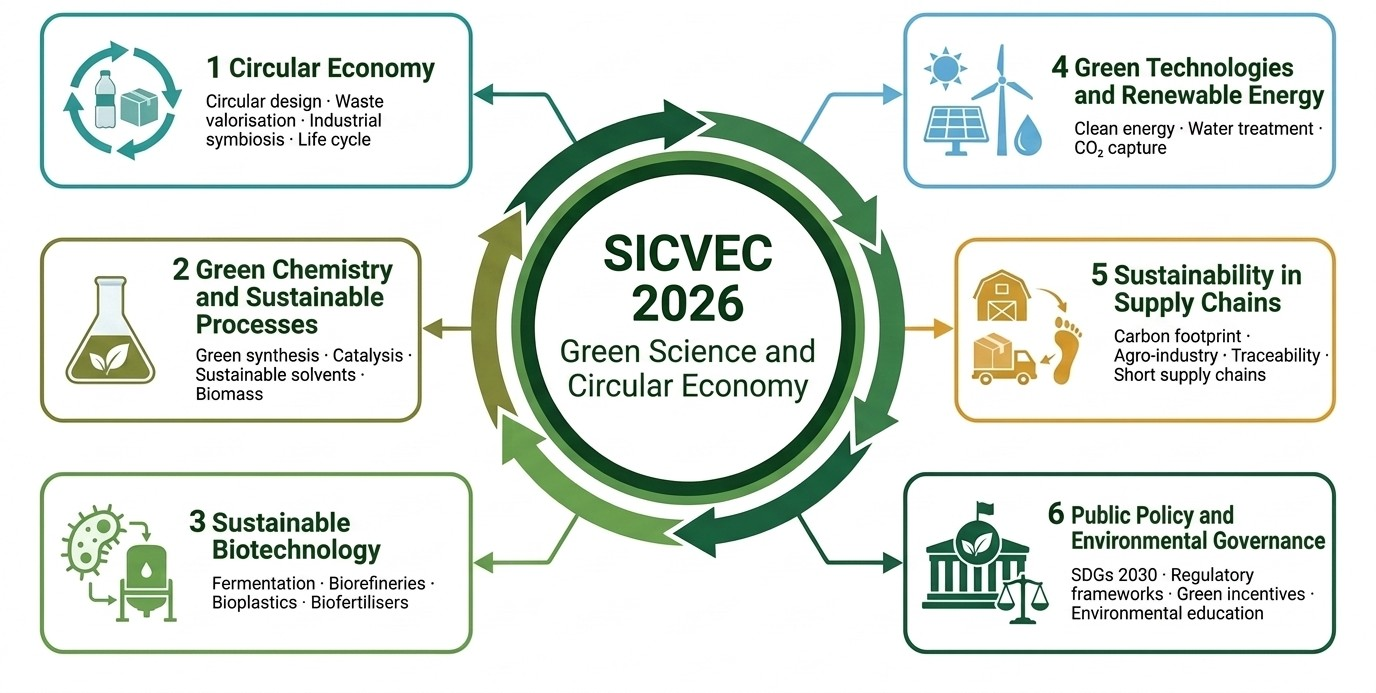
\includegraphics[width=\linewidth]{fig_ejes_en.jpg}

  \vspace{0.2cm}

  \textcolor{dorado}{\textbf{Aligned with SDGs 12, 13, 15, 17}}

  \vspace{0.15cm}

  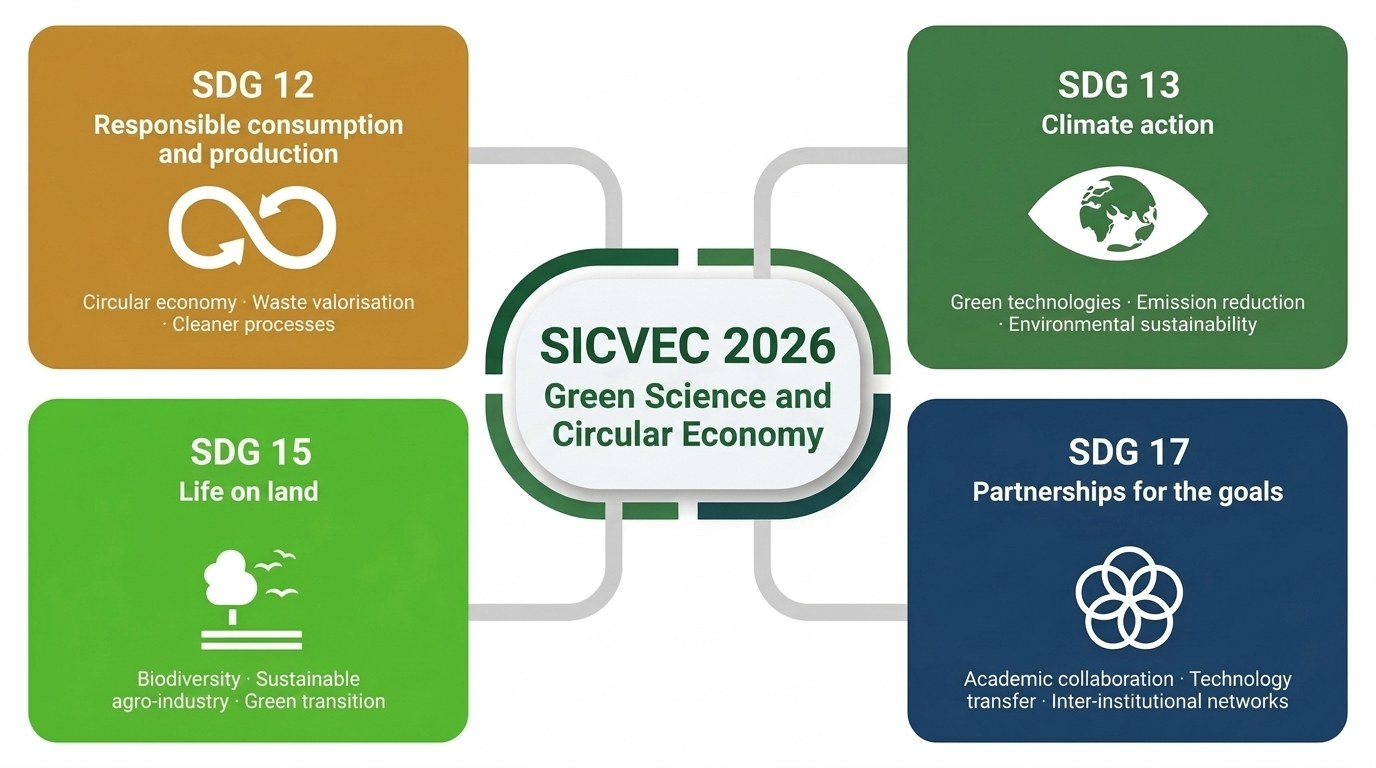
\includegraphics[width=\linewidth]{fig_ods_en.jpg}
\end{minipage}

\vspace{0.12cm}

% ═════════════════════════════════════════════════════════════════════
% CONVOCATORIA
% ═════════════════════════════════════════════════════════════════════

\begin{center}
  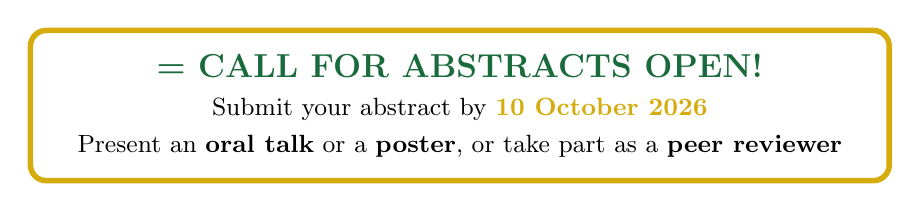
\begin{tikzpicture}
    \node[draw=dorado, line width=2pt, inner sep=0.3cm, rounded corners=0.2cm, fill=blanco] {
      \begin{minipage}{0.85\textwidth}
        \centering
        \textcolor{verdeosc}{\textbf{\large = CALL FOR ABSTRACTS OPEN!}} \\
        \vspace{0.1cm}
        \small Submit your abstract by \textcolor{dorado}{\textbf{10 October 2026}} \\
        \vspace{0.08cm}
        Present an \textbf{oral talk} or a \textbf{poster}, or take part as a \textbf{peer reviewer}
      \end{minipage}
    };
  \end{tikzpicture}
\end{center}

\vspace{0.12cm}

% ═════════════════════════════════════════════════════════════════════
% PÚBLICO OBJETIVO
% ═════════════════════════════════════════════════════════════════════

\begin{center}
  \textcolor{verdeosc}{\textbf{Who is invited?}}

  \vspace{0.1cm}

  {\small Students • Lecturers • Researchers • Professionals in Chemistry, Physics, Biology, Mathematics, Engineering, Environmental Sciences}
\end{center}

\vspace{0.12cm}

% ═════════════════════════════════════════════════════════════════════
% CONTACTO Y ENLACES
% ═════════════════════════════════════════════════════════════════════

\begin{center}
  \textcolor{verdemid}{\textbf{INFORMATION AND CONTACT}}

  \vspace{0.15cm}

  \small
  \textbf{Aldo F. Combariza} — IN SILICO Research Group \\
  → \href{mailto:aldo.combariza@unisucre.edu.co}{\textcolor{verdemid}{aldo.combariza@unisucre.edu.co}} \\

  \vspace{0.1cm}

  → \href{https://sicvec2026.eu.pythonanywhere.com}{\textcolor{verdemid}{sicvec2026.eu.pythonanywhere.com}} \\

  \vspace{0.15cm}

  \href{https://sicvec2026.eu.pythonanywhere.com}{
\includegraphics[width=2.0cm]{qr_web.png}} \\

  \vspace{0.15cm}

  \textcolor{verdeosc}{\textbf{Universidad de Sucre}}

  IN SILICO Research Group — Department of Biology and Chemistry — Faculty of Education and Sciences
\end{center}

\vspace{0.12cm}

% ═════════════════════════════════════════════════════════════════════
% PIE DE PÁGINA
% ═════════════════════════════════════════════════════════════════════

\begin{center}
  \textcolor{dorado}{\textbf{* Sustainable Processes for the Future *}}
\end{center}

\end{document}
